% Preamble
\documentclass{article}


% Packages
\usepackage[legalpaper, portrati, margin=0.9in]{geometry}
\usepackage{amsmath}
\usepackage{bm}
\usepackage{amssymb}
\usepackage{gensymb}
\usepackage{mathtools}
\usepackage[dvipsnames]{xcolor}
\usepackage{caption}
\usepackage{subcaption}
\usepackage{pgfplots}
\pgfplotsset{compat=1.17}
\usepgfplotslibrary{fillbetween}
\usepackage{tikz}
\usepackage{tkz-euclide}
\usepackage{tcolorbox}
\tcbuselibrary{most}
\usepackage{etoolbox}
\AtBeginEnvironment{quote}{\singlespacing\small}
\usepackage{ulem}
\usepackage{cancel}



% Macros
\usepackage{../../../mymacros}


% File Info
\title{PHYS14X Notes}
\author{Eric Xia}
\date{Last Updated 4 October 2020}


% Document
\begin{document}

    \maketitle
    \tableofcontents
    \pagebreak



    \section{Introduction}

    \textbf{Rational:} maximally achieving pre-defined goals; maximizing your expected utility \\
    \textbf{Rationality}: only concerns what decisions are made and not the thought process behind them \\

    Artificial intelligence is often observed in two dimensions, human vs. rational and thought (internal reasoning) vs. behavior (external characterization) \\

    \textbf{Turing Test:} designed as a thought experiment to sidestep the philosophical vagueness of the question "can a machine think?", would need the following capabilities: \\
    $\bullet$ \textbf{Natural language processing} to communicate successfully in a human language \\
    $\bullet$ \textbf{Knowledge representation} to store what it knows or hears \\
    $\bullet$ \textbf{Automated reasoning} to answer questions and to draw new conclusions \\
    $\bullet$ \textbf{Machine learning} to adapt to new circumstances and to detect and extrapolate patterns \\

    \textbf{Total Turing Test:} requires interaction with objects and people in the real world, proposed because Turing viewed the \textit{physical} simulation of a person as unnecessary to demonstrate intelligence,
    the robot would need: \\
    $\bullet$ \textbf{Computer vision:} and speech recognition to perceive the world \\
    $\bullet$ \textbf{Robotics} to manipulate objects and move about \\
    \textbf{Agent:} an entity that operates autonomously, perceives its environment, persists over a prolonged time period, adapts to change, and creates and pursues goals \\
    \textbf{Rational agent:} selects actions that maximize its (expected) utility \\
    \textbf{Limited rationality:} acting appropriately when there is not enough time to do all the computations one might like \\
    \textbf{Value alignment problem:} the values or objectives put into the machine must be aligned with those of the human \\
    \textbf{Incompleteness theorem:} in any formal theory as strong as Peano arithmetic (the elementary theory of natural numbers), there are necessarily true statements that have no proof within the theory \\
    \textbf{Computability:} capable of being computed by an effective procedure \\
    \textbf{Tractability:} a problem is intractable if the time required to solve instances of the problem grows exponentially with the size of the instances \\
    \textbf{NP-completeness:} provides a basis for analyzing the tractability of problems: any problem class to which the class of NP-complete problems can be reduced is likely to be intractable \\
    \textbf{Decision theory:} combines probability theory with utility theory and provides a formal and complete framework for individual decisions made under uncertainty \\
    \textbf{Satisficing:} making decisions that are "good enough" rather than laboriously calculating an exact optimal decision \\


    \section{Foundations}

    \subsection{Representations}

        Visual representations are a vital part of understanding a problem and developing a model. Reprsentations may include pictures, sketches, diagrams, graphs, and a multitude of context-specific procedures.
        To avoid cluttering a reprsentation, it is best to oversimplify a real-life situation and gradually construct less idealized models. It our oversimplified model reproduces the main features of its real-world
        counterpart, then we know we have chosen adequate essential attributes. \\

        \noindent In this respect, mathematical symbols also act as representations of more complex phrases. Take, for example, the statement below.

        \begin{quote}
            "The magnitude of the acceleration of an object is directly proportional to the magnitude of the vector sum of the forces exerted on the object and inversely proportional to the object's inertia.
            The direction of the acceleration is the same as the direction of the vector sum of the forces."
        \end{quote}

        \noindent This can be expressed concisely and more clearly with the mathematic equation,

        \begin{equation*}
            \overrightarrow{a} = \frac{\sum \overrightarrow{F}}{m}
        \end{equation*}


    \subsection{Physical quantities and units}

        \textbf{Physical quantities and their symbols}:

        \begin{center}
            \begin{tabular}{|c|c|}
                \hline
                \textbf{Physical Quantity}  & \textbf{Symbol} \\
                \hline
                length                      & $l$ \\
                \hline
                time                        & $t$ \\
                \hline
                mass                        & $m$ \\
                \hline
                speed                       & $v$ \\
                \hline
                volume                      & $V$ \\
                \hline
                energy                      & $E$ \\
                \hline
                temperature                 & $T$ \\
                \hline
            \end{tabular}
        \end{center}

        \noindent Physical quantities are expressed as the product of a number and a unit of measurement. For example, the length $l$ of an object that is $1.2 m$ long can be expressed as $l=1.2m$. The global unit system
        used in science and engineering is the \textbf{Syst\'eme International (SI)}. There are seven base units in the SI system from which all other units can be derived. \\

        \noindent \textbf{The Seven SI Base Units:}

        \begin{center}
            \begin{tabular}{|c|c|c|}
                \hline
                \textbf{Name of Unit}   & \textbf{Abbreviation} & \textbf{Physical Quantity} \\
                \hline
                meter                   & m                     & length \\
                \hline
                kilogram                & kg                    & mass \\
                \hline
                second                  & s                     & time \\
                \hline
                ampere                  & A                     & electric current \\
                \hline
                kelvin                  & K                     & thermodynamic temperature \\
                \hline
                mole                    & mol                   & amount of substance \\
                \hline
                candela                 & cd                    & luminous intensity \\
                \hline
            \end{tabular}
        \end{center}

        \noindent To work conveniently with very large or very small numbers, we modify the unit name with prefixes representing integer powers of ten, conventionally powers of ten that are multiples of 3. For example,
        a billionth of a second is denoted by 1 ns and pronounced "one nanosecond", where 1 ns $=$ $10^{-9}$s. \\

        \noindent \textbf{SI Prefixes:}

        \begin{center}
            \begin{tabular}{|c|c|c|}
                \hline
                $\bm{10^n}$ & \textbf{Prefix}   & \textbf{Abbreviation} \\
                \hline
                $10^{24}$   & yotta-            & Y \\
                \hline
                $10^{21}$   & zetta-            & Z \\
                \hline
                $10^{18}$   & exa-              & E \\
                \hline
                $10^{15}$   & peta-             & P \\
                \hline
                $10^{12}$   & tera-             & T \\
                \hline
                $10^9$      & giga-             & G \\
                \hline
                $10^6$      & mega-             & M \\
                \hline
                $10^3$      & kilo-             & k \\
                \hline
                $10^0$      & \sout{     }      & \sout{  } \\
                \hline
                $10^{-3}$   & milli-            & m \\
                \hline
                $10^{-6}$   & micro-            & $\mu$ \\
                \hline
                $10^{-9}$   & nano-             & n \\
                \hline
                $10^{-12}$  & pico-             & p \\
                \hline
                $10^{-15}$  & femto-            & f \\
                \hline
                $10^{-18}$  & atto-             & a \\
                \hline
                $10^{-21}$  & zepto-            & z \\
                \hline
                $10^{-24}$  & yocto-            & y \\
                \hline
            \end{tabular}
        \end{center}

        \noindent A \textbf{mole} is currently defined as the number of atoms in $12\times 10^{-3}$ kg of carbon-12. This number is referred to as \textbf{Avogrado's number ($N_A$)}, where the currently accepted
        measurement of Avogradro's number is

        \begin{equation*}
            N_A = 6.0221413 \times 10^{23}
        \end{equation*}

        \noindent \textbf{Density} is the physical quantity measuring how much of some substance exists in a given volume. \textbf{Number density} is the number of objects per unit volume. If there are $N$ objects in a
        volume $V$, then the number density $n$ of these objects is

        \begin{tbhtheorem}{Number Density}
            $n = \frac{N}{V}$
        \end{tbhtheorem}

        \noindent \textbf{Mass density ($\rho$)} is the amount of mass $m$ per unit volume:

        \begin{tbhtheorem}{Mass Density}
            $\rho = \frac{m}{V}$
        \end{tbhtheorem}

        \noindent The easiest way to convert measurements to other units is to write the \textbf{conversion factor} as a fraction. Then multiply what you're to express by the conversion ratio, cancelling out the units.
        Below is an example of converting 4.5 inches to millimeters:

        \begin{equation*}
            4.5 \text{ in. } = (4.5 \cancel{\text{ in. }})\left(\frac{25.4\text{ mm}}{1 \cancel{\text{ in.}}}\right) = 4.5 \times 25.4 \text{ mm } = 1.1 \times 10^2 \text{ mm}
        \end{equation*}


    \subsection{From Reality to Model}

        If the position of an object is not changing, it is said to be \textbf{at rest}. A \textbf{Position-Time Graph} describes the position of an object as a function of a unit of time. Below is a position-time graph
        for walking.

        \begin{center}
            \begin{tikzpicture}[scale= ]
                \begin{axis}[
                    axis lines = center,
                    axis equal image,
                    xlabel = {Distance from origin (mm)},
                    ylabel = {Seconds},
                    xlabel near ticks,
                    ylabel near ticks,
                    xmin = 0,
                    xmax = 20,
                    ymin = 0,
                    ymax = 15,
                    xtick = {0,5,10,15,20},
                    xticklabels = {0,5,10,15,20},
                    ytick = {5,10,15},
                    yticklabels = {5,10,15}
                ]
                \draw[blue](1,2.5) -- (7.5,12.5);
                \draw[red](7.5,12.5) -- (12.5,12.5);
                \draw[ForestGreen](12.5,12.5) -- (19,8);
                \end{axis}
            \end{tikzpicture}
        \end{center}

        \noindent Here, the blue section of the graph describes when the person is walking forwards, the red section is when the person is pausing, and the green section is when the person is walking backwards.
    \section{Motion in One Dimension and Changes in Velocity}

    \subsection{Position and Displacement}
        \textbf{Position-versus-time graph}: a graph that represents position ($x$) as a function of time ($t$).

        \begin{center}
            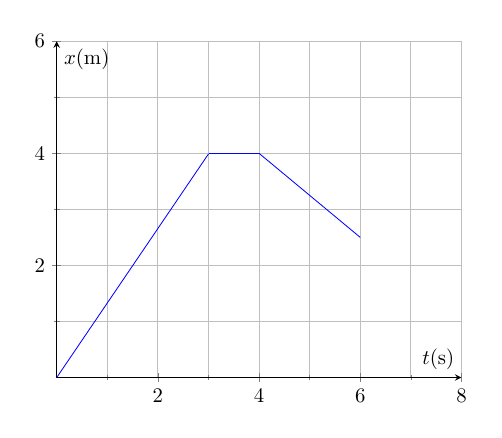
\begin{tikzpicture}[scale=0.75]
                \begin{axis}[
                    axis lines = middle,
                    smooth,
                    xlabel = $t$(s),
                    ylabel =$x$(m),
                    minor tick num =1,
                    grid=both,
                    no markers,
                    domain=0:8,
                    xtick={0,2,4,6,8},
                    ytick={0,2,4,6},
                    xticklabels={0,2,4,6,8},
                    yticklabels={0,2,4,6},
                    xmin=0,
                    xmax=8,
                    ymin=0,
                    ymax=6
                ]
                \addplot[
                    blue,
                    domain=0:3
                ]
                {1.33*x};
                \addplot[
                    blue,
                    domain=3:4
                ]
                {4};
                \addplot[
                    blue,
                    domain=4:6
                ]
                {-0.75*x+7};
                \end{axis}
            \end{tikzpicture}
        \end{center}

        \noindent Here, the object moves forward at a constant velocity between $t=0$ and $t=3$ as demonstrated by the even slope of the curve when $0\leq t\leq 3$. Then the object is at rest between $t=3$ and $t=4$,
        hence the curve is a flat line in that interval. Lastly, the object turns around and moves backward towards the origin, moving at a constant velocity again demonstrated by the even slope of the curve when
        $4\leq t \leq 6$. \\

        \noindent The \textbf{displacement} of an object is the vector change in position. The \textbf{$x$ component of displacement} is given by

        \[
            \Delta x = x_2 - x_1
        \]

        \noindent The particular wording of "$x$ component" reminds us that the $x$ component of displacement is measured along some specific $x$-axis. The $x$ component of displacement can be \textit{either} positive or
        negative. It is positive for displacements in the direction of increasing $x$ and negative for displacements in the direction of decreasing $x$. Whereas \textit{distance traveled} refers to the distance covered
        by a moving object along the path of its motion, \textit{displacement} describes a vector quantity with no reference position or axis. Only when motion is always in the same direction is the distance traveled
        equal to the distance between the initial and final positions.




    \subsection{Representing Motion}
        A curve in a position-versus-time graph is called an $\bm{x(t)}$ \textbf{curve} because it can be represented by a mathematical function $x(t)$.



    \subsection{Average Speed and Average Velocity}
        The slope of an $x(t)$ curve is the speed of the object at that time interval. Hence, in a position-versus-time graph, \textit{the steeper the slope, the higher the speed}.

        \[
            s_{avg} = \frac{\Delta x}{\Delta t}
        \]

        \noindent \textbf{Velocity} is a vector quantity expressing both speed and the direction of travel, where

        \begin{align*}
            x\text{ component of object's } v_{avg} &= \frac{x \text{ component of its displacement}}{\text{time interval for that displacement}} \\
            \Delta x \text{ of object's } v_{avg}   &= \frac{\Delta x \text{ of displacement}}{\Delta t \text{ for displacement}}
        \end{align*}

        \noindent A \textbf{velocity-versus-time graph} represents velocity ($v$) as a function of time ($t$). A curve plotted in such a graph is called a $\bm{v(t)}$ \text{curve}. We denote the $x$ component of an
        object's average velocity by $v_x$.




    \subsection{Scalars and Vectors}
        \textbf{Scalars} are physical quantities specified by a positive or negative magnitude and a unit of measurement. \\
        $\bullet$ e.g. temperature, volume, density, speed, energy, mass, time \\
        $\bullet$ written as a lowercase letter \\

        \noindent \textbf{Vectors} are physical quantities specified by a positive or negative magnitude, a unit of measurement, and a direction in space. \\
        $\bullet$ e.g. force, velocity, acceleration, displacement, momentum \\ \\
        $\bullet$ written as a lowercase letter with a right arrow over it, e.g. $\overrightarrow{v}$

        \noindent The \textbf{magnitude of a vector} is denoted by

        \[
            |\overrightarrow{b}| \text{ or } b
        \]

        \pagebreak

        \noindent To describe vectors mathematically, we use a \textbf{unit vector}, a vector whose sole purpose is to define a direction in space. Unit vectors do not have units and they have a magnitude of 1. Hence,

        \[
            |\hat{i}| = 1
        \]

        \noindent Unit vectors are denoted by a caret/hat ( $\hat{ }$ ) to distinguish them from normal vectors. Unit vectors pointing in the direction of increasing $x$ along the $x$-axis are denoted by
        $\hat{i}$ (pronounced \textit{$i$-hat}). \textbf{Unit vector notation} expresses a vector along the $x$-axis as the product of a scalar and the unit vector:

        \[
            \overrightarrow{b} = b_x \hat{i} \text{  (one dimension)}
        \]

        \noindent where $b_x$ is a scalar known as the $x$ component of $\overrightarrow{b}$. If we take the absolute value of both sides of the above equation, we find that, for vectors in one dimension, the magnitude
        of the vector $\overrightarrow{b}$ equals the magitude of $b_x$:

        \begin{align*}
            \overrightarrow{b}      &= b_x \hat{i} \\
            |\overrightarrow{b}|    &= |b_x \hat{i}| \\
                                    &= |b_x||\hat{i}| \\
                                    &= |b_x|
        \end{align*}

        \noindent If $b_x > 0$ then $\overrightarrow{b}$ is in the same direction as $\hat{i}$. If $b_x < 0$ then $\overrightarrow{b}$ is in the opposite direction to $\hat{i}$.



    \subsection{Position and Displacement Vectors}
        The most basic vector is displacement ($\Delta \overrightarrow{r}$). Recall that the $x$ component of displacement is equal to the change in the $x$ coordinate such that

        \[
            \Delta r_x = \Delta x = x_f - x_i
        \]

        \noindent The distance $d$ between two points is given by

        \[
            d = |x_1 - x_2 | \text{ (one dimension)}
        \]

        \noindent A vector that has zero magnitude is equal to the \textbf{zero vector}, denoted by a zero with an arrow ($\overrightarrow{0}$). In diagrams, the zero vector is represented by a dot. Rearranging the
        definition for $\Delta x$, we get

        \[
            x_f = x_i + \Delta x
        \]

        \noinent An object's position can also be represented by a vector:

        \[
            \Delta x \hat{i} = (x_f - x_i)\hat{i} = x_f \hat{i} - x_i \hat{i}
        \]

        \noindent where the left side of the equation represents the displacement

        \[
            \Delta x \hat{i} = \Delta r_x \hat{i} = \Delta \overrightarrow{r}
        \]

        \noindent The vector $x_i \hat{i}$ represents the \textbf{position vector}, a vector that lets us determine the position of a point in space relative to some chosen origin. Position is also represented by
        $\overrightarrow{r}$:

        \[
            \overrightarrow{r} = x \hat{i} \text{ one dimension}
        \]

        \noindent Hence, we can see that the $x$ component of position is equal to the coordinate such that

        \[
            r_x = x
        \]

        \noindent To subtract a vector from another vector, we reverse the direction of the vector being subtracted and add the reversed vector to the other vector:

        \begin{align*}
            \Delta \overrightarrow{r}  &= \overrightarrow{r_f} - \overrightarrow{r_i \\
                                        &= \overrightarrow{r_f} + (-1)\overrightarrow{r_i}
        \end{align*}

        \noindent The vector $\overrightarrow{a}-\overrightarrow{b}$ can be graphically represented like so:

        \begin{figure*}[hbt!]
            \centering
            \includegraphics[scale=0.75]{Resources/Vector_Subtraction}
        \end{figure*}

        \noindent Scalar multiplication of a vector:

        \[
            c\overrightarrow{a} = c\left(a_x \hat{i}\right) = \left(ca_x\right)\hat{i}
        \]



    \pagebreak
    \subsection{Velocity as a Vector}
        The $x$ component of the average velocity is given by

        \[
            v_{x,av} = \frac{\Delta x}{\Delta t} = \frac{x_f - x_i}{t_f - t_i}
        \]

        \noindent We can multiply the first and middle terms of the above equation by the unit vector $i$ and substitute $\Delta \overrightarrow{r} = \Delta x \hat{i}$ to get

        \[
            \overrightarrow{v_{av}} = v_{x,av}\hat{i} = \frac{\Delta \overrightarrow{r}}{\Delta t}
        \]

        \noindent Because $\Delta t$ is always positive, we see that for one dimensional motion, $\overrightarrow{v_{av}}$ always points in the same direction as displacement.



    \subsection{Motion at Constant Velocity}
        By convention, the phrase "average" is dropped from references to constant velocity. Thus, the $x$ component of the average velocity is simply $v_x$ and we see that the slope of the $x(t)$ curve is numerically
        equal to the $x$ component of the velocity:

        \[
            \frac{\Delta x}{\Delta t} = v_x \text{ constant velocity}
        \]

        \noindent The $x$ component of the displacement during any time interval is given by the area under the $v_x (t)$ curve between the beginning and the end of the time interval. We can use the fact that
        $\Delta x = x_f - x_i$ to rewrite the above equation in terms of $x_f$ such that

        \[
            x_f = x_i + v_x \Delta t \text{ constant velocity}
        \]



    \subsection{Instantaneous Velocity}
        \textbf{Instantaneous Velocity:} the velocity of an object at any given instant. The $x$ component of the velocity at instant $t$ is given by

        \[
            v_x = \lim_{\Delta t\to 0} \frac{\Delta x}{\Delta t} = \frac{dx}{dt}
        \]

        The velocity is then

        \[
            \overrightarrow{v} = v_x \hat{i} = \left(\lim_{\Delta t\to 0} \frac{\Delta x}{\Delta t}\right) \hat{i}
        \]

        Because the unit vector is constant, we can rewrite the velocity as

        \[
            \overrightarrow{v} = \lim_{\Delta t\to 0} \frac{\Delta x \hat{i}}{\Delta t} = \lim_{\Delta t\to 0}\frac{\Delta \overrightarrow{r}}{\Delta t} = \frac{d\overrightarrow{r}}{dt}
        \]

        Hence, speed is given by the magnitude of this vector:

        \[
            v = |\overrightarrow{v}|
        \]

hp

    \subsection{Changes in Velocity}
        \textbf{Acceleration}: the rate of change of velocity with respect to time. The $\bm{x}$ \textbf{component of average acceleration} is the change in the $x$ component of the velocity divided by the time interval
        during which this change took place. In physics, the word "\textit{deceleration}" has no meaning is better avoided, as \textit{acceleration} refers to \textit{any} change in velocity, regardless of increasing
        or decreasing speed. \\

        When an object's velocity and acceleration is in the same direction, the object speeds up. When they are in opposite directions, the object slows down. It is important to note confuse the positive $x$ component
        of acceleration with speeding up when working with objects traveling in the negative $x$ direction. An object speeds up when the magnitude of its velocity (aka speed) increases, regardless of the direction of
        motion. Whether or not the $x$ component of an object's acceleration is positive, however, dependson hte direction in which the object is moving. \\

        \begin{figure}[hbt!]
            \centering
            \caption*{\textbf{Position-versus-time graphs for objects accelerating along the positive $\bm{x}$ axis:}}
            \begin{subfigure}[b]{.45\textwidth}
                \includegraphics[scale=1]{Resources/Position_Time_Graph_Acceleration}
            \end{subfigure}
            \begin{subfigure}[b]{.45\textwidth}
                \includegraphics[scale=1]{Resources/Position_Time_Graph_Acceleration2}
            \end{subfigure}
        \end{figure}

        The curvature of an $x(t)$ curve is a measure of the $x$ component of acceleration. An upward curvature corresponds to a positive $x$ component of acceleration, whereas a downward curvature corresponds to a
        negative $x$ component of acceleration.



    \subsection{Acceleration Due to Gravity}
        In a vacuum, a feather and a stone drop at the same rate. Yet in air, the stone drops faster. This result has been attributed to air resistance pushing harder on the feather than the stone. \textbf{Free fall} is
        the motion of objects moving solely under the influence of gravity. A falling object inside a vacuum is in free fall because it is influenced only by gravity, but an object falling in the air is not in free fall
        because its motion is also affected by air resistance. However, the effect of air resistance on a stone outside of a vacuum is negligible. This property is true for many objects that are not too light and not
        dropped from too great of a height. Hence, if an object is not extremely light or dropped from a substantive height, we can ignore air resistance and consider all dropped objects to be in free fall. \\

        In the absence of air resistance, the \textbf{magnitude of the acceleration of all objects due to gravity} is $\bm{9.8}$ m/$\text{s}^2$ and consequently the amount of \textit{time it takes to fall from a certain height
        is the same for all falling objects.}



    \subsection{Projectile Motion}
        An object that is launched but not self-propelled is a \textbf{projectile}, and its motion is called \textbf{projectile motion}. The path a projectile follows is called its \textbf{trajectory}. The motion of an
        object in free fall is a special case of projectile motion. \\

        Consider a ball launched straight up. The ball slows down as it moves upward and hence its acceleration and velocity point in opposite directions. The ball's velocity changes \textbf{linearly}, changing by
        equal amounts in equal time intervals, thus its acceleration is constant. In the position-versus-time and velocity-versus-time graphs below, it can be seen that the slope of the $v_x (t)$ curve is about
        -10 m/$\text{s}^2$, which is the acceleration due to gravity. Thus, both on the way up and way down, the acceleration of a projectile is equal \textit{both in magnitude and in direction} to that of a freely falling
        object.

        \begin{figure*}[hbt!]
            \centering
            \caption*{$x(t)$ curve for a ball launched straight up:}
            \includegraphics[scale=0.8]{Resources/Projectile_Motion}
        \end{figure*}

        \begin{figure*}[hbt!]
            \centering
            \caption*{$v_x (t)$ curve for a ball launched straight up:}
            \includegraphics[scale=0.9]{Resources/Projectile_Motion2}
        \end{figure*}

        For an object launched upwards, the launch affects only the initial velocity. Once the object is released, the rest of its motion is determined by gravity alone (free fall). At the top of a trajectory of a ball
        launched upwards, there is instant at which the $x$ component of the velocity is zero. \textit{The $x$ component of the acceleration is not zero at the top}. To conceptualize this, consider the graph below.

        \begin{figure*}[hbt!]
            \centering
            \includegraphics[scale=0.6]{Resources/Nonzero_Acceleration_Trajectory}
        \end{figure*}

        Though velocity is zero at the apex of the trajectory, acceleration is defined as

        \[
            a = \frac{dv}{dt}
        \]

        The gradient of the line in the graph is nonzero and happens to be -9.81 m/$\text{s}^2$. Hence, the magntiude of the acceleration does not depend on $v$ and is equal to 9.81 m/$\text{s}^2$ for all values of $v$.



    \subsection{Motion Diagrams}
        \textbf{Motion diagrams} represent the positions of a moving object at equally spaced time intervals. We can make a motion diagrams by the following steps: \\

        1. Use dots to represent the moving object at even time intervals. If the object moves at constant speed then the dots are evenly spaced. Conversely, if the object speeds up, the spacing between the dots
        increases. If the object slows down, the spacing decreases. \\
        2. Choose an $x$ (position) axis convenient for the problem. This is usually an axis that has its origin at the initial or final position of the object and is oriented in the direction of motion or acceleration. \\
        3. Specify the position and velocity at all relevant interests, particularly, the \textbf{initial conditions}— position and velocity at the beginning of the time interval of interest, and the
        \textbf{final positions}— position and velocity at the end of that time interval. Additionally, specify all positions where the velocity reverses direction or the acceleration changes. Label any unknown
        parameters with a question mark. \\
        4. Indicate the acceleration of the object between all instants specified in step 3. \\
        5. To consider the motion of more than one object, draw separate diagrams side by side, one for each object, using one common $x$-axis. \\
        6. If the object reverses direction, separate the motion diagram into two parts, one for each direction of travel. \\

        An acronym for a useful checklist of a motion diagram is "\textbf{VENUS}": \\
        $\bullet$ \textbf{V}ectors and scalars used appropriately \\
        $\bullet$ \textbf{E}verything answered \\
        $\bullet$ \textbf{N}o unknowns left \\
        $\bullet$ \textbf{U}nits correct \\
        $\bullet$ \textbf{S}ignificant digits justified \\

        \begin{figure*}[hbt!]
            \centering
            \caption*{\textbf{A Motion Diagram:}}
            \includegraphics{Resources/Motion_Diagram}
        \end{figure*}




    \subsection{Summary of Symbols and Meanings in This Topic}

    \begin{center}
        \begin{tabular}{|c|c|}
            \hline
            \textbf{Symbol} & \textbf{Meaning} \\
            \hline
            $t$             & clock reading = instant in time \\
            \hline
            $\Delta t = t_f - t_i$  & change in clock reading = interval of time \\
            \hline
            $x$             & $x$-coordinate \\
            \hline
            $d=|x_1 - x_2|$ & straight-line distance between two points (never has sign) \\
            \hline
            $\hat{i}$       & unit vector defining direction of $x$-axis (vector magnitude 1) \\
            \hline
            $\overrightarrow{b} = v_x \hat{i}$  & vector and unit vector notation \\
            \hline
            $b_x$           & $x$ component of vector $\overrightarrow{b}$ (can be positive or negative) \\
            \hline
            $b=|\overrightarrow{b}|=|b_x|$  & magnitude of vector $\overrightarrow{b}$ (always positive) \\
            \hline
            $g=|\overrightarrow{a}_\text{free fall}|= 9.8$ m/$\text{s}^2$  & acceleration due to gravity near Earth's surface \\
            \hline
        \end{tabular}
    \end{center}

    \begin{center}
        \begin{tabular}{|c|c|c|c|}
            \hline
            \textbf{Vector} & \textbf{Meaning} & \textbf{Component} & \textbf{Meaning} \\
            \hline
            $\Delta \overrightarrow{r} = \Delta r_x \hat{i}$    & displacement & $\Delta r_x = \Delta x$    & $x$ component of displacement = change in $x$-coordinate \\
            \hline
            $\overrightarrow{r} = r_x \hat{i}$  & position & $r_x = x$  & $x$ component of position = $x$-coordinate \\
            \hline
            $\overrightarrow{v_{av}}=v_{x,av}\hat{i}$ & average velocity & $v_{x,av} = \frac{\Delta x}{\Delta t}$ & $x$ component of average velocity \\
            \hline
            $\overrightarrow{v} = v_x \hat{i}$ & (instantaneous) velocity   & $v_x = \lim_{\Delta t\to 0} \frac{\Delta x}{\Delta t} = \frac{dx}{dt}$ & $x$ component of (instantaneous) velocity \\
            \hline
            $\overrightarrow{a} = a_x \hat{i}$ & acceleration & $a_x = \frac{\Delta v_x}{\Delta t} = \frac{dv_x}{dt} = \frac{d^2 x}{dt^2}$ & $x$ component of acceleration \\
            \hline
        \end{tabular}
    \end{center}

    \textbf{Average Velocity}: The constant velocity required to achieve the same displacement in the same time interval as the actual motion.

    \[
        v_{avg} = \frac{1}{t_2 - t_1} \int^{t_2}_{t_1} v(t) dt
    \]

    Note that this is just the average value of a function integral.
    \section{Constant Acceleration}

    \subsection{Motion with Constant Acceleration}
        For an object moving with constant acceleration, the $v_x (t)$ curve is a straight line. We know $\Delta v_x$ and $v_{x,f}$ to be

        \begin{align*}
            \Delta v_x  &= v_{x,f}-v_{x,i} = a_x \Delta t & \text{ (constant acceleration)} \\
            v_{x,f}     &= v_{x,i} + a_x \Delta t         & \text{ (constant acceleration)}
        \end{align*}

        We also know displacement to be the area under a velocity curve:

        \begin{figure*}[hbt!]
            \centering
            \includegraphics[scale=0.8]{Resources/Constant_Acceleration}
        \end{figure*}

        Hence, the displacement is given by the area of the triangle and the area of the rectangle. The area of the triangle is

        \[
            \frac{1}{2}(v_{x,f}-v_{x,i})(t_f-t_i)=\frac{1}{2}\Delta v_x \Delta t = \frac{1}{2} a_x(\Delta t)^2
        \]

        and the area of the rectangle is

        \[
            (v_{x,i}-0(t_f-t_i)=v_{x,i}\Delta t
        \]

        Thus, the combined displacement is

        \[
            x_f - x_i = v_{x,i} \Delta t + \frac{1}{2} a_x (\Delta t)^2 \text{ (constant acceleration)}
        \]

        Below are \textbf{kinematics graphs for the three basic types of motion:}

        \begin{figure*}[hbt!]
            \centering
            \includegraphics{Resources/Motion_Diagram2}
        \end{figure*}


    \pagebreak
    \subsection{Free-fall Equations}
        Magnitude of \textbf{acceleration due to gravity (g)} is given by

        \[
            g = |\overrightarrow{a}_{\text{free fall}}|
        \]

        If an object is dropped from a certain height with zero initial velocity along an upward-pointing $x$ axis, then,

        \begin{align*}
            x_f &= x_i - \frac{1}{2} gt^2_f \\
            v_{x,f} &= -gt_f
        \end{align*}

        Example of a Free-fall Diagram:

        \begin{figure*}[hbt!]
            \centering
            \includegraphics[]{Resources/Free_Fall_Diagram}
        \end{figure*}



    \subsection{Inclined Planes}
        \textit{When a ball rolls down an incline starting from rest, the ratio of the distance traveled to the square of the amount of time needed to travel that distance is constant}. For example, if a ball released
        from position $x_i=0$ at $t_1=0$ reaches position $x_1$ at instant $t_1,x_2$ at $t_2$, and $x_3$ at $t_3$, then

        \[
            \frac{x_1}{t^2_1}=\frac{x_2}{t^2_2}=\frac{x_3}{t^2_3}
        \]

        Recall that for an object moving with constant acceleration and starting from rest, we have

        \[
            x_f = \frac{1}{2} a_x t^2_f
        \]

        Hence,

        \[
            \frac{x_f}{t^2_f} = \frac{1}{2} a_x
        \]

        As incline increases, so does the ratio $\frac{x_0}{t^2_0}$. Through experimentation, we can determine the component of acceleration along the incline to be related to $g$ by the equation

        \[
            a_x = g\sin\theta
        \]




    \subsection{Instantaneous Acceleration}
        \[
            a_x = \lim_{\Delta t \to 0} \frac{\Delta v_x}{\Delta t}
        \]

        Hence,

        \[
            a_x = \frac{dv_x}{dt} = \frac{d}{dt} \left(\frac{dx}{dt}\right) = \frac{d^2 x}{dt^2}
        \]

        We can then express changes in velocity and position as:

        \begin{align*}
            \Delta v_x   &= \int^{t_f}_{t_1} a_x (t) dt \\
            \Delta x     &= \int^{t_f}{t_i} v_x (t)dt
        \end{align*}



    \subsection{Summary of Topic}
        \textbf{Free fall}: the motion of an object subject to only the influence of gravity \\
        \textbf{Motion diagram:} a diagram that shows the position of a moving object at equally spaced time intervals and summarizes what is known about the object's initial and final conditions (its position, velocity,
        and acceleration) \\
        \textbf{Projectile motion}: the motion of an object that is luanched but not self-propelled (\textit{projectile}) \\
        $\bullet$ The launch only affects the object's initial velocity \\
        $\bullet$ Once the object is launched, its motion is determined by gravity only, hence \textit{the object is in free fall on the way up as well as on the way down} \\
        \textbf{Trajectory:} the path taken by a projectile \\

        For motion at constant acceleration, the $x$-coordinate and the $x$-component of the velocity of an object are given by

        \begin{align*}
            x_f     &= x_i + v_{x,i} \Delta t + \frac{1}{2} a_x (\Delta t)^2 \\
            v_{x,f} &= v_{x,i} + a_x \Delta t
        \end{align*}

    % Something I found really interesting while reading this chapter was that, when a projectile is at the top of its trajectory, though its velocity is zero, its acceleration has a nonzero value.
This is because acceleration does not depend on instantaneous velocity. I personally found the verbal explanation to be confusing, and only understood after visually representing it. Consider the graph below:

\begin{center}
    \begin{tikzpicture}
        \begin{axis}[
            axis lines = middle,
            axis equal image,
            ylabel = {$v_x$ (m/s)},
            ylabel style = {above left},
            xlabel = {$t$(s)},
            xmin = 0,
            xmax = 8,
            ymin = -2,
            ymax = 2,
            ticks = none
        ]
        \draw[red] (4,0);
        \node[fill=red, draw, circle, minimum width=4pt, inner sep=0pt, pin={[fill=white, outer sep=1pt]60:{\color{red}Peak of Trajectory}\color{black}}] at (4,0) {};
        \addplot[
            color = blue,
            domain = 0:8
        ]
        {-0.5*x+2};
        \end{axis}
    \end{tikzpicture}
\end{center}

We know acceleration to be defined as the gradient of the velocity curve:

\[
    a = \frac{dv}{dt}
\]

Since the $v_x (t)$ curve is linear for scenario of projectile motions, $\frac{dv}{dt}$ is constant for the entire domain of our $v_x (t)$ curve and it happens to be -9.81 m/$\text{s}^2$. This tells us that not only
is the magnitude of acceleration nonzero throughout the entire trajectory, including the peak, but the acceleration is always in the direction of decreasing $x$.
    \section{Momentum}

    \subsection{Friction}

        \textbf{Friction}: the resistance to motion that one surface or object encounters when moving over another. \\
        In the absence of friction, objects moving along a horizontal track keep moving without slowing down.


    \subsection{Inertia}

        \textbf{Inertia}: a measure of an object's tendency to resist any change in its velocity. \\
        $\bullet$ The motion of larger objects made of the same material is harder to change than the motion of smaller objects \\
        $\bullet$ The ratio of the inertias of the two carts is equal to the inverse of the ratio of their velocity changes

    \subsection{What Determines Inertia?}

        \textit{The inertia of an object is determined entirely by the type of material of which the object is made and by the amount of that material contained in the object.}


    \subsection{Systems}

        \textbf{System}: any object or group of objects that we can separate, in our minds, from the surrounding environment \\
        \textbf{Extensive quantities:} quantities whose value is proportional to the size or "extent" of the system \\
        $\bullet$ Only four values can change the value of an extensive quantity: input, output, creation, and destruction \\
        $\bullet$ If we can divide the system into a number of pieces then the sum of an extensive quantity for all the separate pieces is equal to the value of that quantity for the entire system \\
        $\bullet$ The number of trees in a park is extensive because if we divide the park into two parts and add the number of trees in each part then we obtain the number of trees in the park \\
        $\bullet$ The price per gallon of gasoline is not an extensive quantity because we can divide a tankful of gas into two parts and add the price per gallon for the two parts, thus obtaining twice the price per
        gallon for the entire tank \\

        \textbf{Intensive Quantities:} quantities that do not depend on the extent of the system \\
        \textbf{System Diagrams:} diagrams that show a system's intitial and final conditions \\

        The change in the number of trees over a certain time interval is not

        \[
            \text{change } = \text{ final tree count } - \text{ initial tree count}
        \]

        but rather

        \[
            \text{change } = \text{ input - output + creation - destruction}
        \]

        \textbf{Conserved}: any extensive quantity that cannot be created nor destroyed \\
        Hence, the value of a conserved quantity can only change by

        \[
            \text{change } = \text{ input - output}
        \]



    \subsection{Inertial Standard}

        \text{Inertia:} \\
        $\bullet$ A scalar quantity \\
        $\bullet$ Denoted by $m$ \\
        $\bullet$ Represented in kilograms \\

        Recall that the ratio of the inertias of two colliding objects is the inverse of the ratio of the magnitude of their velocity changes. Hence,

        \[
            \frac{m_u}{m_s} = -\frac{\Delta v_{s,x}}{\DElta v_{u,x}}
        \]

        therefore

        \[
            m_u = -\frac{\Delta v_{s,x}}{\Delta v_{u,x}} m_s.
        \]

        Because in the case of colliding objects, the velocities are in opposite directions, the minus sign cancels out and \textit{inertia is then always a positive quantity}. We can substitute the standard quantity
        $m_s=1$ kg into the equation to get

        \[
            m_u = -\frac{\Delta v_{s,x}}{\Delta v_{u,x}} \text{ kg}
        \]



        \subsection{Momentum}

            \textbf{Momentum}: the product of the inertia and the velocity of an object, represented by $\overrightarrow{p}$ and the SI units "kg $\cdot$ m/s":

            \[
                \overrightarrow{p} = m\overrightarrow{v}
            \]

            The $x$ component of the momentum is the product of the inertia and the $x$ component of the velocity:

            \[
                p_x = mv_x
            \]

            Inertia is an intrinsic property of an object (inertia cannot be changed without changing the object) but the value of the momentum of an object can change. With the definition of momentum, we have also
            the equation below, which describes how the change in momentum for an object is always the negative of the change in momentum for another object in a collision.

            \[
                \Delta p_{u,x} + \Delta p_{s,x} = 0
            \]

            This can also be written in vector form:

            \[
                \Delta \overrightarrow{p}_u + \Delta \overrightarrow{p}_s = \overrightarrow{0}
            \]



        \subsection{Isolated Systems}

            The momentum of a system of two moving carts is the sum of the momenta of the two individual carts:

            \[
                \overrightarrow{p} = \overrightarrow{p}_1 + \overrightarrow{p}_2.
            \]

            \textbf{Interaction:} two objects acting on each other in such a way that one or both are accelerated \\
            \textbf{External Interactions:} interactions across the boundary of a system \\
            \textbf{Internal Interactions:} interactions between two objects inside the system \\
            \textbf{Isolated System:} a system for which there are no external interactions

        \subsection{Conservation of Momentum}

            In an isolated system, the momentum of the system is not changing:

            \[
                \Delta \overrightarrow{p} = \overrightarrow{0} \text{ (isolated system)}
            \]

            Thus, for any object that collides with the inertial standard on a level, low-friction track, regardless of initial velocities and values of inertias $m_1$ and $m_2$, we have

            \begin{align*}
                \Delta \overrightarrow{p}_1 + \Delta \overrightarrow{p}_s &= \overrightarrow{0} \text{ (by definition)} \\
                \Delta \overrightarrow{p}_2 + \Delta \overrightarrow{p}_2 &= \ovrerightarrow{0} \text{ (by definition)}
            \end{align*}

            In a system that is not isolated, we have

            \[
                \Delta \overrightarrow{p} = \overrightarrow{J},
            \]

            where $\overrightarrow{J}$ represents the transfer of momentum from the environment to the system, also known as the \textbf{impulse} delivered to the system. Like momentum, impulse is a vector and has units
            of kg $\cdot$ m/s.

        \subsection{Lecture 6 Notes}

            Inertia is actually the same thing as gravitational mass. \\

            For collisions, we have

            \[
                \frac{m_1}{m_2} = -\frac{\Delta \overrightarrow{v}_2}{\Delta \overrightarrow{v}_1}
            \]

            When you choose a system, be consistent and keep note of: \\
            $\bullet$ Interactions: pushing/pulling that can change motion of object, if the interactions cross the system boundary then they are \textit{external} \\
            $\bullet$ Isolation: no external interactions or external interactions are mutually cancelled or external interactions are negligible (at least temporarily) \\

            Whereas systems in biology have to be interacting, systems in physics can be literally anything. Systems in physics don't need to be interacting or even have the same properties. \\

            \[
                \Delta \text{Quantity } = J + A,
            \]

            where $J$ is transfer (I-O) and $A$ is creation - destruction. If the system is isolated, then $J=0$ (nothing crosses system boundary). If a quantity cannot be created nor destroyed, it is said to be
            conserved. \\

            We have

            \[
                \Delta \overrightarrow{p}_{sys}= \overrightarrow{J},
            \]

            where $\overrightarrow{J}$ is impulse. Because impulse is simply a change in momentum, the units for impulse are the same as momentum. \\

            In general,

            \[
                \overrightarrow{p}_{sys} = \sum^n_{i=1} \overrightarrow{p}_i
            \]


        \subsection{Topic Summary and Equations}

            For collisions between identical objects on level surfaces,

            \[
                \Delta \overrightarrow{v}_1 = -\Delta \overrightarrow{v}_2
            \]






    \section{Kinetic and Internal Energy}

    \subsection{Classification of Collisions}


        \textbf{Relative velocity:}
        \begin{align*}
            \overrightarrow{v}_{12} = \overrightarrow{v}_2 - \overrightarrow{v}_1 \text{ is velocity of cart 2 relative to cart 1} \\
            \overrightarrow{v}_{21} = \overrightarrow{v}_1 - \overrightarrow{v}_2 \text{ is velocity of cart 1 relative to cart 2}
        \end{align*}

        $v_{12}$ is velocity of cart 2 and $v_{21}$ is velocity of cart 2. \textbf{Relative speed} is the magnitude of the relative velocity.

        \textbf{Elastic Collision}: a collision in which the relative speed before the collision is the same as the relative speed after the collision \\
        $\bullet$ collisions between hard objects are usually elastic \\

        \textbf{Inelastic Collision:} a collision for which the relative speed after the collision is lower than that before the collision \\
        \textbf{Totally Inelastic Collision:} a special case of an inelastic collision in which the two objects move together after the collision so that their relative speed is reduced to zero \\



    \subsection{Kinetic Energy}

        \textbf{Kinetic energy}: energy associated with a single object's motion, extensive property (depend on amount of matter being measured), given by

        \[
            K = \frac{1}{2} mv^2
        \]

        \textit{In a typical elastic collision, the sum of the kinetic energies of the objects before the collision is the same as the sum of the kinetic energies after the collision.} \\

        Because kinetic energy is a scalar extensive quantity, bar diagrams are a good way to visually represent changes in this quantity:

        \begin{figure*}[hbt!]
            \centering
            \includegraphics[]{Resources/Kinetic_Energy}
        \end{figure*}



    \subsection{Internal Energy}

        \textbf{State}: the condition of an object as specified by some complete set of physical parameters: shape temperature, whatever - \textit{every possible physical variable that defines the object}. \\
        In inelastic collisions, objects deform and heat up. A \textbf{process} is a transformation of a system from an initial state to a final state. Inelastic collisions are \textbf{irreversible processes}.
        Elastic collisions are \textbf{reversible processes}. \\

        The energy of a system is given by the sum of the \textit{kinetic} and \textit{internal} energies:

        \[
            E = E_K + E_{int}
        \]

        \begin{figure*}[hbt!]
            \centering
            \includegraphics[scale=0.5]{Resources/Collisions}
        \end{figure*}

        \textit{In any inelastic collision, the states of the colliding objects change and the sum of their internal energies increases by an amount equal to the decrease in the sum of their kinetic energies. The energy
        of a system of two colliding objects does not change during the collision.} \\

        \textbf{Law of Conservation of Energy:} Energy can be transferred from one object to another or converted from one form to another, but it cannot be destroyed or created.


    % \section{Conservation of Energy}

    \subsection{Closed Systems}

        \textbf{Closed system}: any system to or from which no energy is transferred \\
        $\bullet$ a closed system need not be isolated \\

        Below are some energy bar diagrams for initial and final conditions:

        \begin{figure*}[hbt!]
            \centering
            \includegraphics[]{Resources/Energy_Bar_Closed_System}
        \end{figure*}



    \subsection{Elastic Collisions}

        For elastic collisions, the objects \textit{relative speed},

        \[
            v_{12} = |\overrightarrow{v}_2 - \overrightarrow{v}_1|
        \]

        is the same before and after the collision. For two objects moving along the $x$ axis, we can write this as

        \[
            v_{2x,i} = v_{1x,i} = -(v_{2x,f} - v{1x,f})
        \]

        Recall that \texxtbf{kinetic energy} is given by

        \[
            K = \frac{1}{2} mv^2
        \]

        Thus, for elastic collisions,

        \[
           K_i = K_F \equiv \Delta K = 0
        \]

        Kinetic energy is represented in \textbf{joules}, where

        \[
            1 \text{ kg } \cdot \text{ m}^2\text{/s}^2 = 1 \text{ J}
        \]



    \subsection{Inelastic Collisions}

        The majority of collisions are between the two extremes of elastic and totally inelastic. For these cases, we can define the ratio of relative speeds as the \textbf{coefficient of restitution ($e$)}:

        \[
            e = \frac{v_{12f}}{v_{12i}}
        \]

        Because $e$ is a ratio of speeds which are always positive, $e$ is also always positive. We generally write $e$ with a negative value because the relative velocity changes sign after the collision:

        \[
            e = - \frac{v_{2x,f} - v_{1x,f}}{v_{2x,i} - v_{1x,i}} = - \frac{v_{12,f}}{v_{12x,i}}
        \]

        \begin{figure*}[hbt!]
            \centering
            \includegraphics[scale=0.75]{Resources/Coeff_Of_Restitution}
        \end{figure*}



    \subsection{Conservation of Energy}

        The combined kinetic and internal energies of a system is given by

        \[
            E = K + E_{int}
        \]

        For a closed system, we have

        \[
            \Delta E_{int} = -\Delta K
        \]


    \subsection{Explosive Separations}

        \textbf{Explosive separation}: where objects separate or break apart from each other \\
        $\bullet$ kinetic energy increases and internal energy decreases in these cases

    \subsection{Topic Summary}

        \textbf{Closed system:} a system to or from which no energy is transferred \\
        \textbf{Coefficient of restitution ($\bm{e}$)} (unitless): A scalar equal to the ratio of relative speeds after and before a collision of two objects:

        \[
            e = \frac{v_{12f}}{v_{12i}}
        \]

        \textbf{Conservation of energy:} energy can be transferred from one object to another or converted from one form to another, but it cannot be created or destroyed. The energy of a closed system cannot change:

        \[
            \Delta E = 0 \text{ (closed system)}
        \]

        \textbf{Elastic, inelastic, totally inelasic collisions:} collisions between two objects are classified according to what happens to the relative speed

        \[
            v_{12} = |\overrightarrow{v}_2 - \overrightarrow{v}_1|
        \]

        of the two objects. \\

        \textbf{Energy, E(J)}: A scalar that provides a quantitative measure of the state or motion of an object or system. Energy appears in many different forms. The energy of an object or system always refers to the
        sum of all forms of energy in that object or system. \\
        \textbf{Explosive separation:} a process in which objects break apart from one another and the relative speed of the objects increases. \\
        \textbf{Internal Energy, $\bm{E}_{int}$ (J)}: any energy not associated with the motion of an object or system. Internal energy is a quantitative measure of the state of the object or system. \\
        \textbf{Irreversible process:} a process involving changes that cannot undo themselves spontaneously. \\
        \textbf{Joule (J)}: The derived SI unit of energy, defined as

        \[
            1 J = 1 \text{ kg } \cdot \text{ m}^2\text{/s}^2
        \]

        \textbf{Process}: the transformation of a system from an intial state to a final state \\
        \textbf{Relative Velocity, $\bm{\overrightarrow{v}_{12}}$ (m/s)}: The velocity of one object relative to another:

        \[
            \overrightarrow{v}_{12} = \overrightarrow{v}_2 - \overrightarrow{v}_1
        \]

        The magnitude of this velocity is called the \textbf{relative speed}:

        \[
            v_{12} = |\overrightarrow{v}_2 - \overrightarrow{v}_1}
        \]

        \textbf{Reversible process}: a process that can run backward so that the initial state is restored \\
        \textbf{State}: The condition of an object (or a system) as specified by a complete set of variables



\end{document}